% Preámbulo
% Preámbulo
\documentclass[stu, 12pt, letterpaper, donotrepeattitle, floatsintext, natbib]{apa7}
\usepackage[utf8]{inputenc}
\usepackage{comment}
\usepackage{marvosym}
\usepackage{graphicx}
\usepackage{float}
\usepackage{amsmath}
\usepackage[normalem]{ulem}
\usepackage[spanish]{babel} 
\usepackage{indentfirst} %para le formato que quiere la profe QUITAR SI QUIERES OG APA7
\usepackage{ragged2e} %para le formato que quiere la profe QUITAR SI QUIERES OG APA7
\usepackage{indentfirst} %para le formato que quiere la profe QUITAR SI QUIERES OG APA7
\usepackage{multirow,booktabs,setspace,caption} %formato de figuras APA
\DeclareCaptionLabelSeparator*{spaced}{\\[2ex]}
\DeclareCaptionLabelSeparator*{spaced}{\\[2ex]}
\captionsetup[figure]{textfont=it,format=plain,justification=justified,
  singlelinecheck=false,labelsep=spaced,skip=0pt}

\selectlanguage{spanish}
\useunder{\uline}{\ul}{}
\newcommand{\myparagraph}[1]{\paragraph{#1}\mbox{}\\}

% Portada
%\thispagestyle{empty}
\title{\Large Tarea 3 Unidad 4: Ejemplos de aplicación de Interpolado, Gourand y Phong}
\author{Abraham Jhared Flores Azcona} % (autores separados, consultar al docente)
% Manera oficial de colocar los autores:
%\author{Autor(a) I, Autor(a) II, Autor(a) III, Autor(a) X}
\affiliation{Instituto Tecnológico de Tijuana}
\course{SCC-1010SC5C: Graficación}
\professor{Dra. Martha Elena Pulido}
\duedate{26 de octubre de 2021}

\begin{document}
    % Índices
    \pagenumbering{arabic}
    \maketitle

    % Cuerpo 
    %NOTA: PARA CITAR ESTILO "Merts (2003)" usar \cite{<nombre_cita_bib>}
    %    
    \newpage
    \section{Ejemplos de aplicación}
    \vspace{\baselineskip}
    \subsection{Interpolado}
    \subsubsection{Concepto}
    Es aquella \begin{justifying}
      cuando un objeto con superficies planas (bajo ciertas condiciones)
      puede sombrearse realísticamente utilizando las intensidades de superficie constantes.
      Llegara el caso en donde una superficie se expone solamente a la luz ambiente y no se aplica
      diseños, texturas ó sombras de superficie, el sombreado constante genera una representación exácta
      de la superficie \citep{unknown-author-2021}.\par
    \end{justifying}
    \vspace{\baselineskip}
    \subsubsection{Ejemplo}
    \begin{figure}[H]
      \centering
      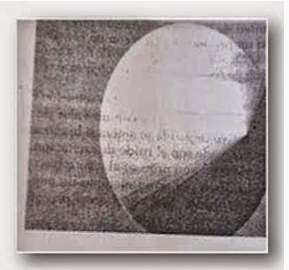
\includegraphics[width=8cm,height=6cm]{object_intrpolation.JPG}
      \caption{Este objeto está sombreado con interpolado.}
    \end{figure}
    \vspace{\baselineskip}
    \subsection{Gouraud}
    \subsubsection{Concepto}
    Esta \begin{justifying}
      se basa en interpolación de intensidad. Consideran que facetas planas colindantes proceden
      de la aproximación de las superficies cúrvas; elimina las discontinuidades de iluminación, es más sipmle
      pero con peores resultados en objetos de brillo especular, y es implementado en OpenGL \citep{garcia-2021}.\par
    \end{justifying}
    \vspace{\baselineskip}
    \subsubsection{Ejemplo}
    \begin{figure}[H]
      \centering
      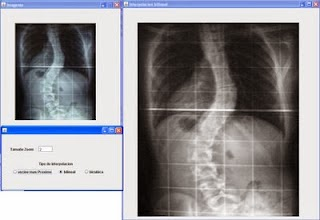
\includegraphics[width=10cm,height=6cm]{xray_gourand.jpg}
      \caption{Una aplicación es aquella de las imágenes de rayos X.}
    \end{figure}
    \vspace{\baselineskip}
    \subsection{Phong}
    \subsubsection{Concepto}
    Es \begin{justify}
      una técnica de interpolación que obtiene el sombreado de las superficies en gráficos 3D computarizados.
      Calcula las normas de cada vértice, interpola en cada pixel de los polígonos rasterizados para finalmente calcular el color
      del pixel basándose en la norma interpolada y el método de interpolación \citep{unknown-author-no-date}.\par
    \end{justify}
    \vspace{\baselineskip}
    \subsubsection{Ejemplo}
    \begin{figure}[H]
      \centering
      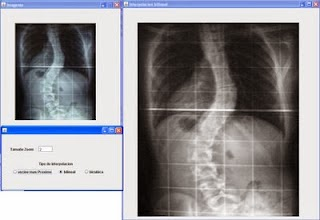
\includegraphics[width=10cm,height=6cm]{xray_gourand.jpg}
      \caption{Se compara un objeto con sombreado plano con otro con sombreado Phong.}
    \end{figure}
    \vspace{\baselineskip}
    \newpage   
    % Referencias
    \renewcommand\refname{\textbf{Referencias}}
    \bibliography{referencias}
    
\end{document}